\chapter{ndnSIM}

Named Data Networking (NDN) is a newly proposed Internet communication paradigm that tries to keep most of the well accepted and tested TCP/IP Internet architecture (as shown in \ref{fig:NetworkStack}), while evolving the thin waist introducing many new features \cite{ndn17}. These features differ in fundamental ways from a point-to-point communication architecture and need to be simulated extensively under constantly changing parameters and implementations \cite{Ajunwadkar14}.

NdnSIM is an open source simulator for NDN networks within the existing NS-3 simulator framework. Its main goals are to facilitate experimentation inside the research community and make all basic NDN protocol operations accessible and therefore changeable like routing, data caching, packet forwarding and congestion management \cite{mastorakis16}. Packet-level interoperability with CCNx implementation is given in order to support traffic measurements, traffic traces and analysis tools between CCNx and ndnSIM. Large-scale simulations should be supported and made easy to set up through helper classes. Helper classes automate the repetitive creation of single entities like nodes and set them up in a standardized way. Therefore, the simulator has been implemented in a very modular fashion making it very easy to modify, replace or re-implement specific components like the FIB, PIT or forwarding strategy. Replacing components have minimal or no impact on other components, as long as they adhere to the modules API's and other components they interact with \cite{Afanasyev16}.

\newpage

\section{Design overview}

NS-3 and ndnSIM both follow a philosophy of maximum abstraction for all modeled components making experimentation on one hand very fine-grained and on the other hand very isolated and decoupled from the rest. The NDN core protocol stack can be installed on every simulated network node in a consistent manner through helpers, that take care of all the parts that need to play together like the inter-node communication with installed applications through their respective application faces.

\vspace{5mm} %5mm vertical space

\begin{figure}[H]
  \centering
  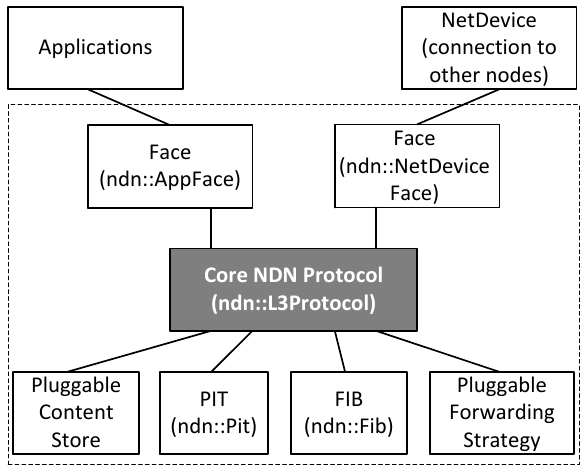
\includegraphics[scale=0.4]{chapter-3/ndnSIMcomponentAbstraction}
  \caption{Basic component abstractions in ndnSIM \cite{afanasyev12}}
  \label{fig:ndnSIMcomponentAbstraction}
\end{figure}

\vspace{5mm} %5mm vertical space

The basic component abstractions are seen in figure \ref{fig:ndnSIMcomponentAbstraction}. The core NDN Protocol is the ndn::L3Protocol that receives interest and data packages from upper and lower layers through the corresponding faces. As of ndnSIM version 2.0 there are two distinct faces: the application face (ndn::AppFace) is responsible for inter-node communication between the application and the node itself while the net device face (ndn::NetDeviceFace) is responsible for inter-network communication with different nodes. Other faces for different purposes are expected to be added by the core developer or the community as needed. The CS (ndn::ContentStore) is an abstraction for in-network caching of data and can easily be omitted or replaced by another implementation of a different storing policy. The PIT (ndn::Pit) abstracts the data structure that is responsible for logging all received interests with their nonce and incoming faces while the FIB (ndn::Fib) abstracts the data structure to guide the strategy in interest forwarding. The Strategy (ndn::ForwadingStrategy) is responsible for implementing how interests and data are forwarded. That includes lookups in the content store for cached data, in PIT for already forwarded interests and in FIB if both previous searches didn't yield any matches. Each action in the forwarder of the strategy is represented as a virtual function in the forwarder header class and can be overwritten.

\subsection{Face Abstraction}

The face abstraction plays an important role in the overall modularity of the NDN simulator by acting as an interface, therefore, making ndnSIM design independent from any underlying transport layers. All communication between application, the NDN core protocol and other nodes with the L3 protocol happens through faces that take care of any needed conversion.

\vspace{5mm} %5mm vertical space

\begin{figure}[H]
  \centering
  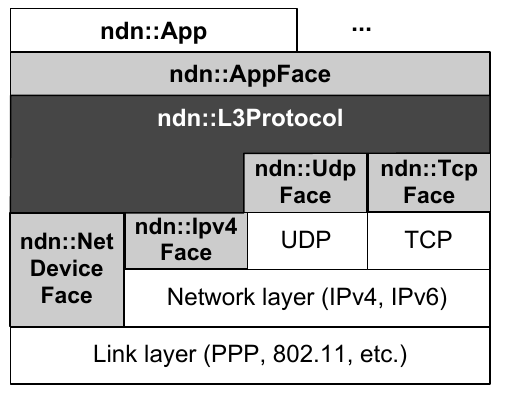
\includegraphics[scale=0.4]{chapter-3/CommunicationLayerAbstraction}
  \caption{Face abstractions around ndn::l3Protocol \cite{afanasyev12}}
  \label{fig:CommunicationLayerAbstraction}
\end{figure}

\vspace{5mm} %5mm vertical space

As shown in \ref{fig:CommunicationLayerAbstraction} the application can communicate with ndn::L3Protocol through the AppFace whereas for inter-node transmission it depends on the transmission protocols which faces need to be used. TCP and UDP have their respective ndn::UdpFace and ndn::TcpFace. IPv4 and IPv6 also have their own ndn::Ipv4Face making it particularly easy to implement the NDN architecture on top of IP or even TCP/IP. If NDN needs to be implemented without TCP/IP protocol it can communicate directly with the link layer through the ndn::NetDeviceFace.

\subsection{Content Store Abstraction}

The CS is crucial for the NDN Internet architecture as it caches data for later use in potentially all the intermediate nodes. It can do rudimentary error recovery and multicast the data asynchronously downstream to the requesters. The replacement policy determines what data is saved into cache and how it gets replaced or deleted after a certain time. Currently implemented versions of the CS support Least Recently Used (ndn::cs::Lru), First In First Out (ndn::cs::Fifo) and a Random Replacement Policy (ndn::cs::Random). Each implementation is based on a dynamic trie-based data structure with hash-based indexing as are the PIT and FIB implementations.

\subsection{Pending Interest Table (PIT) Abstraction}

The PIT data structure keeps information about each forwarded interest. Each PIT entry is uniquely identified by the content name of the interest. It holds a list of all incoming faces on which the interest was received and a list of all outgoing faces that the interest has been forwarded to. The arrival and expiration time are also kept in order to retransmit a lost interest. The nonce of an interest is a randomly generated number that is attached to the interest and identifies the interest in order to avoid loops. Nonce and Interest name uniquely identify the interest. Different consumers issuing the same interest will very likely have different nonces. In that case, no loop is detected and the incoming face is added to the already existing PIT entry. If the same nonce and interest are received again, the interest has looped and should be dropped.

\vspace{5mm} %5mm vertical space

\begin{figure}[H]
  \centering
  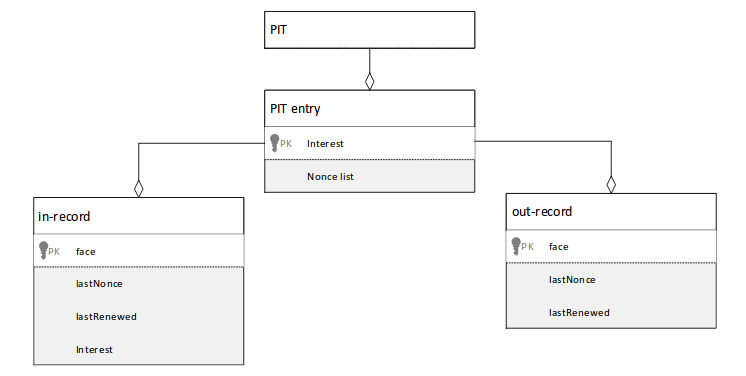
\includegraphics[scale=0.4]{chapter-3/PITdataStructure}
  \caption{PIT data structure \cite{Afanasyev16}}
  \label{fig:PITdataStructure}
\end{figure}

\vspace{5mm} %5mm vertical space

Figure \ref{fig:PITdataStructure} shows the different PIT classes and how they relate to each other. There are also two additional timers on every PIT entry that are not explicitly shown here. The \emph{unsatisfy timer} is the lifetime of an interest and counts down. If it reaches 0 the PIT entry has expired and needs to be forwarded again. The \emph{straggler timer} starts counting down as soon an interest got rejected or satisfied. The straggler timer gives the node the time to detect further loops by the satisfied or rejected interest still floating within the network. Also, data plane measurements of returning data might require to still finish obtaining data points just after that event. Deleting the PIT entry immediately, there would be no means to detect loops and acquire valuable measurements \cite{Afanasyev16}. After the straggler timer runs out the PIT entry is deleted. The PIT abstraction provides basic functions to insert, lookup, delete PIT entries and get measurements if necessary.

\newpage

\subsection{Forwarding Information Base (FIB) Abstraction}

The FIB guides the forwarding strategy in making decisions about Interest forwarding. It is similar to an IP's FIB but contains name prefixes instead of IP prefixes and holds several interfaces (out-faces) therefore enabling multicast forwarding. The faces are ordered according to their cost (routing metric) putting the cheapest connections at the beginning of the list. The lookup is performed on the content name prefixes. The longest prefix match yields the requested FIB entry with its outgoing face(es).

\vspace{5mm} %5mm vertical space

\begin{figure}[H]
  \centering
  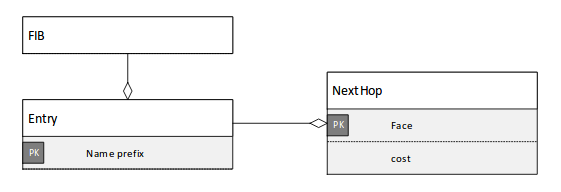
\includegraphics[scale=0.4]{chapter-3/FIBdataStructure}
  \caption{FIB data structure \cite{Afanasyev16}}
  \label{fig:FIBdataStructure}
\end{figure}

\vspace{5mm} %5mm vertical space

As shown in Figure \ref{fig:FIBdataStructure} each FIB entry that has been identified by longest-prefix match has an aggregated collection of NextHops. The NextHop collection must be non-empty and for every NextHop there is one outgoing face towards a possible content source. There may only be one NextHop with a specific face id. The FIB abstraction provides basic insertions, deletions, and exact match operations.

\subsection{Forwarding Strategy Abstraction}

NdnSIM's modular architecture allows experimenting with different types of forwarding strategies without having to adapt any core components. The forwarder class interacts with the strategy and has the following important functions:

\begin{itemize}
\item \emph{onIncomingInterest}: checks for localhost violations and if the interests have looped. Then the function inserts or updates the PIT, resets its timers and looks if the interest can be satisfied by cached data.
\item \emph{onContenStoreMiss}: if there is no data to satisfy the interest, the strategy is called.
\item \emph{onOutgoingInterest}: this function is called by the strategy and forwards the interest to the outgoing faces.
\item \emph{onIncomingData}: checks for localhost violations and if there are any PIT entries for that data. If there are no PIT entries the data is dropped, otherwise, the data will be handed on to the onOutgoingData function.
\item \emph{onOutgoingData}: forwards the data downstream towards the content requester.
\end{itemize}


The strategy is called on three occasions. The first time from the forwarder::onContentStoreMiss(), when the decision has to be made how to forward the interest upstream. The second time from the forwarder::onContentStoreHit() to decide how to proceed with a satisfied interest. And the last time from the forwarder::onIncomingData()

\vspace{5mm} %5mm vertical space

The strategy has one important function:

\begin{itemize}
\item \emph{afterReceiveInterest}: it receives the interest and the corresponding FIB and PIT entries from the forwarder and decides how to forward them further and through which faces.
\end{itemize}


\section{Simulation Environment}

The NS-3 simulator supports several simulation environments. In this thesis, NS-3 PyViz was used as a live simulator \cite{pyviz}. PyViz also has an interactive console that visualizes the connections between the nodes of the simulation. It also can be used to debug the state of the running object, show PIT and FIB entries in live and where packages are being dropped.

\vspace{5mm} %5mm vertical space

\begin{figure}[H]
  \centering
  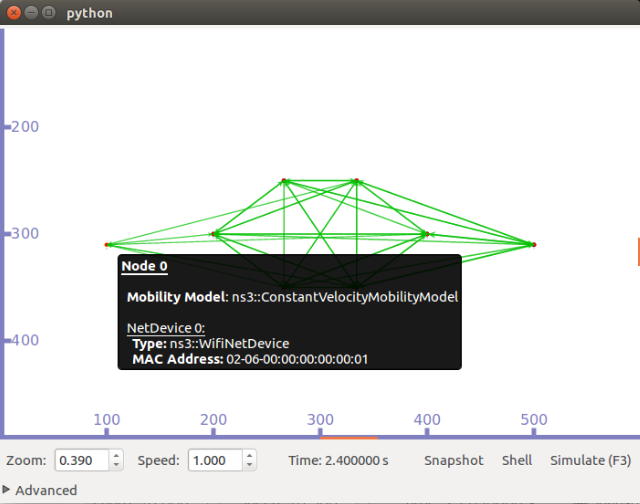
\includegraphics[scale=0.4]{chapter-3/Simulation}
  \caption{Simulation of a possible scenario}
  \label{fig:Simulation}
\end{figure}

\vspace{5mm} %5mm vertical space

Figure \ref{fig:Simulation} shows a current scenario in development. Zoom and speed can interactively be adjusted. The simulation can be started and paused at any time. Node-specific information can be shown while hovering over the node. Traffic between the nodes is visualized by green lines. The current utilized bandwidth is mentioned just above the traffic lines in a live simulation.

\vspace{5mm} %5mm vertical space

\begin{figure}[H]
  \centering
  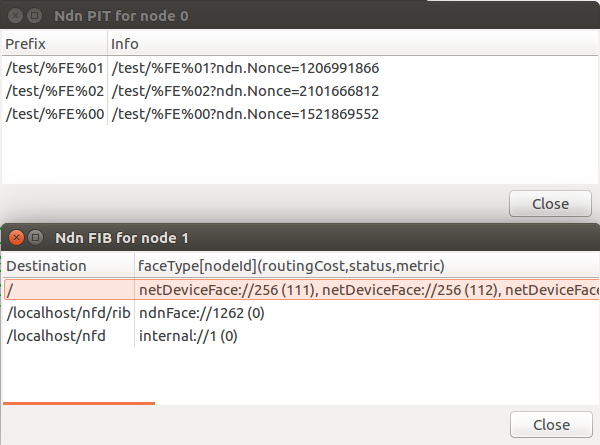
\includegraphics[scale=0.4]{chapter-3/PITandFIBvis}
  \caption{PIT and FIB entries in real time}
  \label{fig:PITandFIBvis}
\end{figure}

\vspace{5mm} %5mm vertical space

Figure \ref{fig:PITandFIBvis} shows all the PIT and FIB entries in real time. Face id's with the corresponding face type are also shown for easier debugging purposes.

\section{Forwarding by the NDN Forwarding Daemon (NFD)}

\vspace{5mm} %5mm vertical space

All the above mentioned modular components and abstractions are implemented and coordinated by the NDN Forwarding Daemon (NFD), which is a network forwarder that implements and evolves with the NDN protocol. NFD is responsible to correctly forward interest and data packages, maintain all basic data structures like CS, PIT and FIB, and implement the packet processing logic. Management interfaces are used by NFD to configure, control and monitor the different components.

\vspace{5mm} %5mm vertical space

Packet processing in NFD is accomplished through forwarding pipelines and forwarding strategies. A forwarding pipeline is an aggregation of different steps that are applied on a packet or a PIT entry. Forwarding pipelines are triggered by specific events like the reception of an Interest, detection of a loop, of when an interest is ready to be forwarded further, etc. A forwarding strategy is attached at the beginning or the end of a pipeline and supports it with information about how and when to forward the interest. Figure \ref{fig:PipelinesAndStrategies} shows the interactions between forwarding pipelines and strategies. For the thesis, relevant pipelines will be shortly described.

\vspace{5mm} %5mm vertical space

\begin{figure}[H]
  \centering
  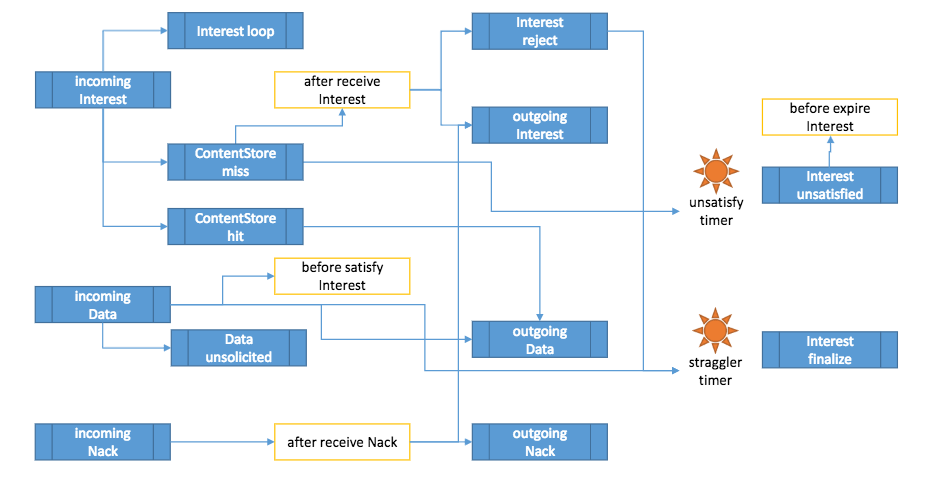
\includegraphics[scale=0.4]{chapter-3/PipelinesAndStrategies}
  \caption{Pipelines and Strategies, white boxes are decision points inside the strategy while blue boxes represent the different pipelines \cite{Afanasyev16}}
  \label{fig:PipelinesAndStrategies}
\end{figure}

\vspace{5mm} %5mm vertical space

Forwarding pipelines operate on interests, data and nacks (negative acknowledgments send downstream to inform about the failure to satisfy a particular interest). After a pipeline has finished it's processing, the packet is handed off to another pipeline or to a decision point inside the strategy until all processing is finished. NFD uses three main forwarding paths:

\begin{itemize}
\item \emph{Interest Processing Path}
\item \emph{Data Processing Path}
\item \emph{Nack Processing Path}
\end{itemize}

The first two paths will be explained further. The nack processing path has not yet been implemented in ndnSIM 2.0 and is under active investigation, therefore it will not be explained.

\subsection{Interest Processing Path}

The interest processing path consists of the following pipelines:

\begin{itemize}
\item \emph{incoming interest}: Interest has been received through a face and is ready to be processed by the forwarder
\item \emph{interest loop}: loop has been detected and interest needs to be dealt with
\item \emph{content store miss}: incoming interest cannot be satisfied by the content store
\item \emph{content store hit}: incoming interest can be satisfied by CS and does not need further forwarding 
\item \emph{outgoing interest}: interest is made ready and sent out
\item \emph{interest reject}: strategy rejects interests according to PIT entries
\item \emph{interest unsatisfied}: processing unsatisfied PIT entries before timeout
\item \emph{interest finalize}: deletion of PIT entries
\end{itemize}

\subsubsection{Incoming Interest Pipeline}

After receiving an interest package through a face implemented in \texttt{Face::onReceiveInterest} the interest is forwarded to the incoming interest pipeline that is implemented in \texttt{Forwarder::onIncomingInterest} method. The input parameters to this method are the interest itself and a reference to the face it was received on. Figure \ref{fig:IncomingInterestPipeline} shows all the steps taken within the pipeline.

\vspace{5mm} %5mm vertical space

\begin{figure}[H]
  \centering
  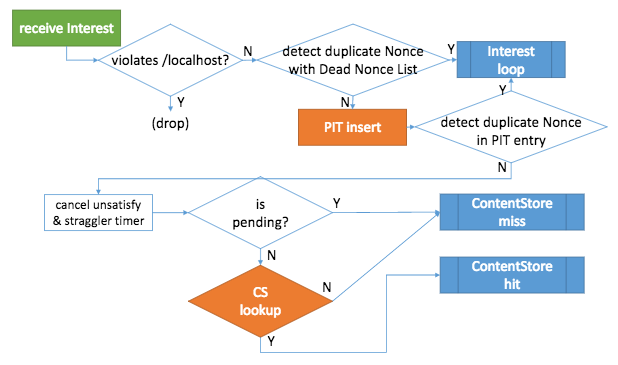
\includegraphics[scale=0.5]{chapter-3/IncomingInterestPipeline}
  \caption{Pipelines and Strategies, white boxes are decision points inside the strategy while blue boxes represent the different pipelines \cite{Afanasyev16}}
  \label{fig:IncomingInterestPipeline}
\end{figure}

\vspace{5mm} %5mm vertical space

The following is a short step by step description of the pipeline in figure  \ref{fig:IncomingInterestPipeline}:

\begin{enumerate}
\item An interest reaching the node through a non-local face is not allowed to have the \texttt{\\localhost} prefix since this prefix is reserved for localhost communication only. This check is necessary because interests with the \texttt{\\localhost} prefix can be used to configure the node and make unwanted changes. The compliant forwarder has no reason to send such an interest to a non-local face.
\item Next the name of the interest with its nonce is checked against the dead nonce list. That happens before the PIT entry is created for the incoming interest (supplements the regular nonce checking through PIT entries). If the tuple of interest and nonce have been processed already, the incoming interest has been looped and will be handed off to the interest loop pipeline.
\item Using the name and the selectors of the interest the PIT is searched for matches. If no match can be found a new PIT entry is created, otherwise an existing PIT entry is updated with the new information mainly the inFace and timers. In Figure \ref{fig:SimpleInterestForwarding} of chapter 2 the CS was checked first, then the PIT was searched and created if necessary. NFD has a slightly different approach. It is expected that the CS will be much larger than the PIT. A search in the CS may take much longer than a PIT lookup, and if a pending interest is present the CS lookup can be omitted saving time and resources.
\item The nonce of the interest is checked against the nonces in the PIT and if a loop or multi-path arrival is detected the interest will be handed off to the interest loop pipeline. If no loop or multi-path arrival is detected the forwarding process is continued.
\item Since a new valid interest arrived and the PIT entries got updated, the current unsatisfy timer (fires when the PIT entry expires) and the straggler timer (fires when PIT entry is no longer needed after it has been satisfied or rejected) are canceled.
\item This step checks if the interest is pending (if the PIT entry has already another in-record from the same or different face).
\item If there is no PIT entry a CS lookup is needed in order to satisfy the interest (ContentStore hit) or forward it (ContentStore miss). If there is already a pending interest the CS lookup has been done already on a previous interest that led to a PIT entry since no match could be found.
\end{enumerate}

\subsubsection{ContentStore Miss Pipeline}

If the ContentStore lookup in \texttt{Forwarder::onIncomingInterest} doesn't yield any data that can satisfy the interest, the content store miss pipeline is called. This pipeline is implemented in \texttt{Forwarder::onContentStoreMiss} and the parameters for this method are the interest packet, the incoming face and the PIT entry. The validity of the interest has been checked already and it needs to be forwarded by taking the following steps:

\begin{enumerate}
\item In the incoming interest pipeline a PIT entry was created already. Now the in-record with its incoming face needs to be added to the PIT entry and if it already exists then the in-record with its face is updated. The expiration counter is set to the value of the interest's field \texttt{InterestLifetime}.
\item The PIT entry's unsatisfy timer is set. It will expire as soon as all in-records of this entry have expired and hand control off to the interest unsatisfied pipeline.
\item The content store miss pipeline then decides which strategy to use and forwards the interest with its incoming face and PIT entry to the chosen strategy for further processing.
\end{enumerate}

The incoming interest pipeline has finished.

\subsubsection{ContentStore Hit Pipeline}

If the ContentStore lookup in \texttt{Forwarder::onIncomingInterest} does yield a match, the content store hit pipeline is called through its implementation in \texttt{Forwarder::onContentStoreHit}. The parameters include the interest packet, incoming face, the PIT entry and the data. The straggler timer is being set since the interest is about to be satisfied. After that, the data is handed off to the outgoing data pipeline.

The incoming interest pipeline has finished.

\subsubsection{Outgoing Interest Pipeline}

The \texttt{Forwarder::onOutgoingInterest} method implements the outgoing interest pipeline. It is entered from the \texttt{Strategy::sendInterest} or a child of the Strategy class that overrides the method. The parameters are the PIT entry, the outgoing face and a \texttt{wantNewNonce} boolean that signalizes that a new nonce is needed for the interest. As mentioned above the PIT entry holds a reference to the interest and therefore the interest packet is not in the parameters list. Figure \ref{fig:OutgoingInterestPipeline} illustrates the outgoing interest pipeline.

\vspace{5mm} %5mm vertical space

\begin{figure}[H]
  \centering
  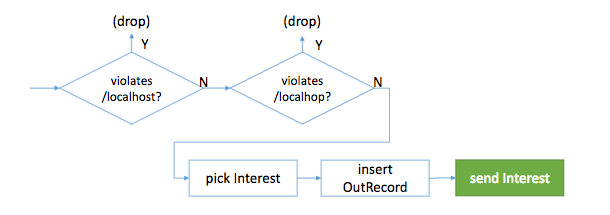
\includegraphics[scale=0.5]{chapter-3/OutgoingInterestPipeline}
  \caption{Outgoing interest pipeline \cite{Afanasyev16}}
  \label{fig:OutgoingInterestPipeline}
\end{figure}

\vspace{5mm} %5mm vertical space

\begin{enumerate}
\item First localhost and localhop violation is checked. Interests with a /localhost scope are not permitted to be sent out through non-local faces. Interests with a /localhop scope are permitted to be sent out through a non-local face only if the PIT entry has one or more in-records with that has a local face stored in it.
\item The interest is picked from the PIT entry and saved to a local variable.
\item If the \texttt{wantNewNonce} flag is set, the interest is copied and a new nonce is attached to it. This is necessary when the node needs to retransmit the interest. If the interest wouldn't receive a new nonce it would be recognized as a looped interest and dropped immediately.
\item An out-record is created in the PIT entry and add an out-face to it. If an out-record with the same out-face already exists, the entry gets refreshed by the \texttt{InterestLifetime} value.
\item The interest is forwarded upstream via out-face.
\end{enumerate}

\subsection{Data Processing Path}

The data processing path consists of the following pipelines:

\begin{itemize}
\item \emph{incoming data}: incoming data are processed
\item \emph{data unsolicited}: unsolicited (not requested) data are processed
\item \emph{outgoing data}: data is forwarded downstream
\end{itemize}

\subsubsection{Incoming Data Pipeline}

 \texttt{Face::onReceiveData} fires when an data arrives at a face. It triggers the  \texttt{Forwarder::onData} which calls \texttt{Forwarder::onIncomingData} with the incoming face and the data as parameters.
The following figure \ref{fig:IncomingDataPipeline} summarizes the steps taken by this pipeline:

\vspace{5mm} %5mm vertical space

\begin{figure}[H]
  \centering
  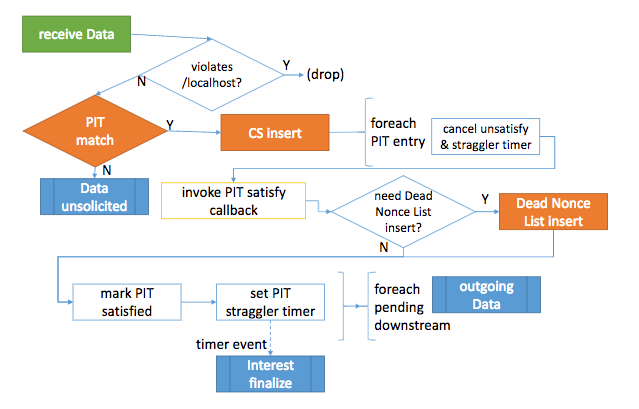
\includegraphics[scale=0.5]{chapter-3/IncomingDataPipeline}
  \caption{Incoming data pipeline \cite{Afanasyev16}}
  \label{fig:IncomingDataPipeline}
\end{figure}

\vspace{5mm} %5mm vertical space

\begin{enumerate}
\item Like with the incoming interest pipeline the /localhost scope needs to be checked. Data may not contain the prefix /localhost when coming from a non-local face.
\item The incoming data needs to be checked against the PIT entries to find out if it is solicited or unsolicited. The data is unsolicited if no matching PIT entry is found. In this case, it is forwarded to the next pipeline: data unsolicited.
\item If one or more PIT entries have been found the data is solicited and therefore inserted into the CS. How the data is processed in the CS is up to the policies defined in the content store.
\item The unsatisfy and straggler timers for all matched PIT entries need to be canceled since the interest is being satisfied.
\item The responsible strategy is determined and triggers the method \texttt{Strategy::beforeSatisfyInterest}. By default, it is empty in ndnSIM 2.0 and can be implemented by a custom strategy overriding the method.
\item The nonce of the data is added to the dead nonce list for further loop detection since interest and data could still be floating inside the network. This is necessary because the next steps delete the corresponding in- and out-records of the PIT entry and the nonce would be lost. 
\item The PIT entry is marked satisfied. All in-records and out-records (corresponding to the incoming face of the data) are being deleted.
\item For every pending downstream the data is handed off to the next pipeline, the outgoing data pipeline, with its corresponding face. NFD takes care that the data is handed off only once for every distinct downstream, even if several PIT entries are found.
\end{enumerate}

\subsubsection{Outgoing Data Pipeline}

The outgoing data pipeline is implemented in \texttt{Forwarder::onOutgoingData} and can be called from two different pipelines. If the incoming interest pipeline found a CS match, the data is fetched and passed to \texttt{Forwarder::onOutgoingData} with the corresponding out-face (the interest's in-face in the PIT entry). If the incoming data pipeline found one or more PIT matches, the data and out-face are passed to this method.

This pipeline has three steps:

\begin{enumerate}
\item The localhost scope is checked. Data with the prefix /localhost are not permitted to be sent out through a non-local face.
\item This step is reserved for traffic management and traffic shaping but not implemented in ndnSIM 2.0 yet.
\item The data packet is sent out through it's out-face.
\end{enumerate}


